\documentclass[10pt,letter]{article}
\usepackage{amsmath}
\usepackage{amssymb}	% packages that allow mathematical formatting
\usepackage{graphicx}
\graphicspath{{../Code/02_Graphs/}}
\usepackage{setspace}	% package that allows you to change spacing
\usepackage{fullpage}	% package that specifies normal margins
\usepackage{microtype}
\usepackage{amsthm}
\newcommand{\argmin}{\operatornamewithlimits{argmin}}
\renewcommand\qedsymbol{$\blacksquare$}
\usepackage{listings,lstautogobble}
\lstset{language=R,
	autogobble=true,
	breaklines=true
}
\usepackage{pgfplotstable} %include csv tables
\usepackage{float} %allows specific table positionings
\usepackage{color}

\definecolor{codegreen}{rgb}{0,0.6,0}
\definecolor{codegray}{rgb}{0.5,0.5,0.5}
\definecolor{backcolour}{rgb}{0.95,0.95,0.95}

\lstdefinestyle{mystyle}{
	backgroundcolor=\color{backcolour},   
	commentstyle=\color{codegreen},
	keywordstyle=\color{blue},
	numberstyle=\tiny\color{codegray},
	stringstyle=\color{cyan},
	basicstyle=\footnotesize,
	breakatwhitespace=false,         
	breaklines=true,                 
	captionpos=b,                    
	keepspaces=true,                 
	numbers=left,                    
	numbersep=5pt,                  
	showspaces=false,                
	showstringspaces=false,
	showtabs=false,                  
	tabsize=2
}

\lstset{style=mystyle}

\usepackage[left=2.5cm, right=2.5cm, top=2cm, bottom = 3cm]{geometry}
	

\begin{document}
\title{FNCE 924 --- Problem Set 2}
\author{Felix Nockher and Patrick Shultz}
\date{\today}
\maketitle 

\section*{Problem 1: Neoclassical Growth Model}

\subsection*{1. What is the long run growth rate of GDP or income?}

Since in steady state (= long run) we have $k^\star = k_{t+1} = k_{t} \forall t$ and $N^\star = N_{t+1} = N_{t} \forall t$ we have $$\frac{A_{t+1}P_{t+1}}{A_{t}P_{t}}=\gamma_A\gamma_P \equiv \gamma$$ as the long run growth rate.

\subsection*{2. Write down the first order conditions for the problem}
We first de-trend the lagrangian by dividing the budget constraint as well as the level-consumption in the utility by $A_t P_t$ using our usual standardization that $P_0 = 1$ and $A_0 = 1$ such that $P_t = \gamma_P^t$ and $A_t = \gamma_A^t$. We denote de-trended variables by their lower-case letters:
\begin{align*}
\mathcal{L} & = \sum^\infty_{t=0} \beta^t P_t \frac{\left[(A_t P_t)^\theta \left( \frac{C_t}{A_t P_t} \right)^\theta (1 - N_t)^{1-\theta} \right]^{1-\sigma}-1}{1-\sigma} +\lambda_t \left[ k_t^{1 - \alpha} (ZN_t)^\alpha -c_t -qk_{t+1}\gamma + q (1-\delta) k_t - g_t\right]\\
 &=\sum^\infty_{t=0} [\beta^\star]^t \frac{\left[ c_t^\theta (1 - N_t)^{1-\theta} \right]^{1-\sigma}-(A_t P_t)^{\theta (\sigma - 1)}}{1-\sigma} +\lambda_t \left[ k_t^{1 - \alpha} (ZN_t)^\alpha -c_t -qk_{t+1}\gamma + q (1-\delta) k_t - g_t\right]\\
 & \text{where } \beta^\star = \beta \gamma_P (\gamma_A \gamma_P)^{\theta(1 - \sigma)}
\end{align*}
$\Rightarrow$ FOCs:
\begin{align*}
[c_t]&\quad \lambda_t = [\beta^\star]^t \theta c_t^{\theta -1 } (1 - N_t)^{1 - \theta}  [c_t^\theta (1-N_t)^{1-\theta}]^{- \sigma}\\
[N_t]&\quad \alpha \left( \frac{k_t}{ZN_t}\right)^{1-\alpha} \lambda_t = [\beta^\star]^t (1-\theta)c_t^\theta(1-N_t)^{-\theta}  [c_t^\theta (1-N_t)^{1-\theta}]^{- \sigma}\\
[k_{t+1}]&\quad 1 = \frac{\lambda_{t+1}}{\lambda_t}\frac{1}{q\gamma}[\underbrace{(1-\alpha) k_{t+1}^{-\alpha}(ZN_{t+1})^\alpha}_{\equiv \text{ net return to capital $r_k$}} + q ( 1 - \delta )]\\
[\lambda_{t}]&\quad k_t^{1 - \alpha} (ZN_t)^\alpha = c_t + qk_{t+1}\gamma - q (1-\delta) k_t + g_t
\end{align*}

\subsection*{3. Calibrate the model}
\begin{align}
\gamma_P &= 1.01 \\
\gamma &= 1.03/\gamma_P = 1.02 \\
\delta &= 0.08 \\
r_k &= 0.05 \\
\alpha &= 2/3 \\
qi^\star &= g^\star = 1/6 y_t \\
N^\star &= 0.35 \\
\sigma &= 4
\end{align}

\subsection*{4. Compute the steady-state level of consumption and capital as a function of your parameter choices and Z}
Solving sequentially for ratios which are constant functions of the model parameters in steady state: 
\begin{align*}
	via\ [k_{t+1}]:&\quad q = \frac{r_k}{\gamma -1 + \delta} = 0.5000\\
	via\ [k_{t+1}]:&\quad \frac{k^\star}{N^\star} = \left[ \frac{(1-\alpha)}{q( \gamma -1 + \delta)} \right]^{1/\alpha} Z= 0.0172*Z\\
	\Rightarrow&k^\star = N^\star * \frac{k^\star}{N^\star} = 0.0060*Z\\
	via\ [\lambda_{t}]\ and\ Eq.\ (6):&\quad \frac{c^\star}{k^\star} = \left( \frac{k^\star}{N^\star} \right)^{-\alpha} Z^\alpha - q\frac{i^\star}{k^\star} - \frac{g^\star}{k^\star}\\
&	\qquad = \left( \frac{k^\star}{N^\star} \right)^{-\alpha} Z^\alpha -2q(\gamma - 1 + \delta) = 14.9000\\
\Rightarrow&c^\star =\frac{c^\star}{k^\star}*k^\star = 0.0898*Z\\
\end{align*}

\subsection*{5. Suppose the productivity parameter Z increases by 10\%. What is the percent increase in consumption and capital?}
As we see above both steady state policies consumption and capital are linear functions in Z and thus a 10\% increase in the latter entails a 10\% increase in the policies.

\subsection*{6. Suppose country X has the same economic parameters as the US, expect for productivity Z and the cost of investment goods q and the share of government spending in GDP which is 25\%}
\subsubsection*{6.i GDP per capita in X 25\% of US and Z is 50\% lower}
With $N_{US}=N_X$ we get:
\begin{align*}
\frac{GDPPC_{US}}{GDPPC_X} &= \frac{\gamma_A^t y_{US}}{\gamma_A^t y_X}=\frac{y_{US}}{y_X}=4\\
4 &= \left( \frac{k^\star_{US}}{k^\star_X}\right)^{1-\alpha} \left( \frac{Z_{US}}{0.5Z_{US}} \right)^\alpha\left(\frac{N_{US}}{N_X}\right)^\alpha\\
&=\left[\frac{N^\star_{US}Z_{US}\left(\frac{1-\alpha}{q_{US}(\gamma-1+\delta)}\right)}{N^\star_{X}0.5Z_{US}\left(\frac{1-\alpha}{q_{X}(\gamma-1+\delta)}\right)}\right]^{1-\alpha} 2^\alpha \left(\frac{N_{US}}{N_X}\right)^\alpha\\
\Rightarrow2 &= \frac{q_X}{q_{US}}
\end{align*}
\subsubsection*{6.ii Local government of X lowers q by 10\%}
 \begin{align*}
 \frac{y_{US}}{y_X} &= \left[\frac{N^\star_{US}Z_{US}\left(\frac{1-\alpha}{q_{US}(\gamma-1+\delta)}\right)}{N^\star_{X}0.5Z_{US}\left(\frac{1-\alpha}{0.9*2q_{US}(\gamma-1+\delta)}\right)}\right]^{1-\alpha} 2^\alpha \left(\frac{N_{US}}{N_X}\right)^\alpha\\
  &= 2*\frac{1.8q_{US}}{q_{US}} = 3.6
 \end{align*}
So now the GDPPC of X is 27.78\% of the US, a 2.78p.p. increase.

\newpage

\section*{Problem 2: Long Run Growth and the Rate of Return on Capital}
\subsection*{1. What is the growth rate of wage income and thus the stock of human capital in this economy?}
Consider the firm's problem 
\begin{equation}
	\mathcal{L} = \sum_{s = 0}^{\infty}\beta^s \frac{\lambda_{t+s}}{\lambda_t}\left(K_{t+s}^{1-\alpha}(ZA_{t+s}P_{t+s}N_{t+s})^\alpha -  N_{t+s}W_{t+s} - I_{t+s} - q_{t+s}\left[K_{t+s+1}-(1-\delta)K_{t+s}-I_{t+s}\right]\right)
	\label{eq:firm_problem}
\end{equation}
The first order condition with respect to $N_{t+s}$ implies 
\begin{equation*}
	\frac{\lambda_{t+s}}{\lambda_t} \alpha\left[ \frac{K_{t+s}}{ZA_{t+s}P_{t+s}N_{t+s}}\right]^{1-\alpha} (ZA_{t+s}P_{t+s}) = W_{t+s}
\end{equation*}
shifting back $s$ periods gives 
\begin{equation*}
\begin{split}
		 \alpha\left[ \frac{K_{t}}{ZA_{t}P_{t}N_{t}}\right]^{1-\alpha} (ZA_{t}P_{t}) &= W_{t}\\
		 \alpha\left[ \frac{k}{ZN_{t}}\right]^{1-\alpha} (ZA_{t}P_{t}) &= W_{t}\\
\end{split}
\end{equation*}
since we know that the detrended capital to labor ratio is constant, we see that $\gamma_W = \gamma_A \gamma_P \equiv \gamma$. 
\subsection*{2. What is the growth rate of capital?}
To calculate the growth rate of capital, we consider the first order condition of Equation \ref{eq:firm_problem} with respect to capital ($K_{t+s+1}$)
\begin{equation*}
\begin{split}
	\frac{\lambda_{t+s}}{\lambda_t}q_{t+s} &= \frac{\lambda_{t+s+1}}{\lambda_{t+s}}\bigg((1-\alpha)\left[\frac{ZA_{t+s}P_{t+s}N_{t+s}}{K_{t+s+1}}\right]^\alpha + (1-\delta) q_{t+s+1}\bigg)\\
	\frac{\lambda_{t+s}}{\lambda_t}q_{t+s} &= \frac{\lambda_{t+s+1}}{\lambda_{t+s}}\bigg((R^k_{t+1}-1) + (1-\delta) q_{t+s+1}\bigg)\\
\end{split}
\end{equation*}
where $r^k$ denotes the net return to capital. Shifting back $s$ periods 
\begin{equation*}
	q_{t} = \frac{\lambda_{t+1}}{\lambda_{t}}\bigg((R^k_{t+1}-1) + (1-\delta) q_{t+1}\bigg)\\
	\label{eq:FOC_K}
\end{equation*}
The first order condition with respect to investment gives $\frac{\lambda_{t+s}}{\lambda_t}(q_{t+s}-1) = 0$, which implies $q_t = 1$ $\forall t$. Thus, Equation \ref{eq:FOC_K} becomes 
\begin{equation*}
1 = \frac{\lambda_{t+1}}{\lambda_{t}}\bigg((R^k_{t+1}-1) + (1-\delta)\bigg)\\
\end{equation*}

solving for $(R^k_{t+1}-1)$ gives 
\begin{equation*}
	(R^k_{t+1}-1) = \frac{\lambda_t}{\lambda_{t+1}} - (1-\delta) = \delta - 1
\end{equation*}
so the growth rate of capital is constant and is dependent on the depreciation rate in the economy. 
\subsection*{3. Derive an expression for the equilibrium growth rate, $r$, in this economy? What is the sign of $r-g$? Can it be negative?}
Start with the detrended production function $y_t = k_t^{1-\alpha}(ZN)^\alpha$ and take the derivative with respect to $k_t$ to get 
\begin{equation*}
	r_t = (1-\alpha)k_t^{-\alpha}(ZN)^{\alpha}
\end{equation*}
plugging in the steady state of capital from question 1 part 4, we get 
\begin{equation*}
\begin{split}
	r^\star &= (1-\alpha)\left[NZ\bigg(\frac{1-\alpha}{q(\gamma-1+\delta)}\bigg)^{\frac{1}{\alpha}}\right]^{-\alpha}(ZN)^\alpha\\
	&= q(\gamma-1+\delta)
\end{split}
\end{equation*}
which implies 
\begin{equation*}
	\begin{split}
	r - g &= q(\gamma - 1 + \delta)-\gamma +1
	\end{split}
\end{equation*}
Setting the expression above equal to zero, we can solve for a condition for when it is negative versus positive
\begin{equation*}
	q^* = \frac{\gamma-1}{\gamma-1+\delta} = \frac{g}{g+\delta}
\end{equation*}
Thus, when $q>q^*$ the sign of $r-g$ is positive and when $q<q^*$ the sign of $r-g$ is negative. 
\subsection*{4. Suppose population growth declines. What is the impact on the steady-state value of $r-g$? }
\subsection*{5. Suppose average growth rates of population and productivity each decline by $0.5\%$ per year from the previous steady state. What is the quantitative impact of these declines on the steady-state level of the real interest rates? }
\section*{Problem 3: Solow Growth Model}
Consider the following deterministic version of the Solow model:
\begin{equation*}
	c_t + k_{t+1} - (1-\delta)k_t \leq Ak_t^{\alpha}
\end{equation*}
where $k_0 > 0$, consumption is $75\%$ of national income, $\delta = 0.1$, and $\alpha = 1/3$. 
\begin{enumerate}
	\item Compute the steady state level of capital as a function of $A$. For what follows pick $A$ to normalize the steady-state of capital to $1$. \\
	
	\noindent\textbf{Solution:}
	Using the fact that $c_t = \frac{3}{4}Ak_t^\alpha$, imposing equilibrium and noting that $k_{t+1} = k_t$ at steady state, we get the following equation for capital accumulation
	\begin{equation*}
		k - (1-\delta)k = \frac{1}{4}Ak^\alpha
	\end{equation*}
	solving this equation for $k$, we see that 
	\begin{equation*}
		k^\star = \left[\frac{A}{4\delta}\right]^{\frac{1}{1-\alpha}}
	\end{equation*}
	where $\star$ denotes the steady state. To calibrate $A$ such that steady state is normalized to $1$, we solve the following expression for $A$
	\begin{equation}
		1 = \left[\frac{A}{4\delta}\right]^{\frac{1}{1-\alpha}}
		\label{eq:A_calibration}
	\end{equation}
	which implies $A = \frac{2}{5}$. 
	\item Start the economy with an initial capital stock of $0.5$. Compute and plot the equilibrium level of capital over time. How long does it take for the capital stock to reach 0.9?
    \noindent\textbf{Solution:} We use the following capital accumulation equation to simulate the growth path of capital 
    \begin{equation}
    	k_{t+1} -(1-\delta)k_t = \frac{1}{4}Ak_t^\alpha
    	\label{eq:capital_accumulation}
    \end{equation}
    The results are shown in Figure \ref{fig:cap_accumulation_alpha_low}. We see that it takes 25 periods for capital to reach $0.9$. 
    \begin{figure}[!htb]
    	\centering
    	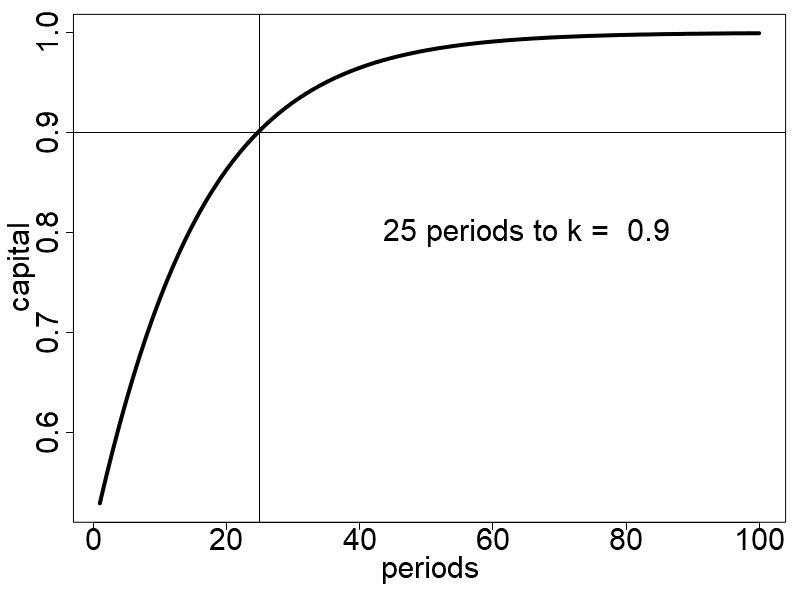
\includegraphics[width=0.5\linewidth]{solow_growth_alpha_low.png}
    	\caption{Capital accumulation with $\alpha = 1/3$}
    	\label{fig:cap_accumulation_alpha_low}
    \end{figure}
	\item Now suppose $\alpha = 2/3$. Recompute the steady-state and again normalize $A$ to ensure that $k=1$ at the steady-state. \\
	
	\noindent\textbf{Solution:} Inspecting Equation \ref{eq:A_calibration}, we see that changing $\alpha$ does not change the level of $A$ required to normalize the steady-state of capital to $1$. We once again use Equation \ref{eq:capital_accumulation} to specify the growth of capital in our economy. The results are shown in Figure \ref{fig:cap_accumulation_alpha_high}.
	\begin{figure}[!htb]
		\centering
		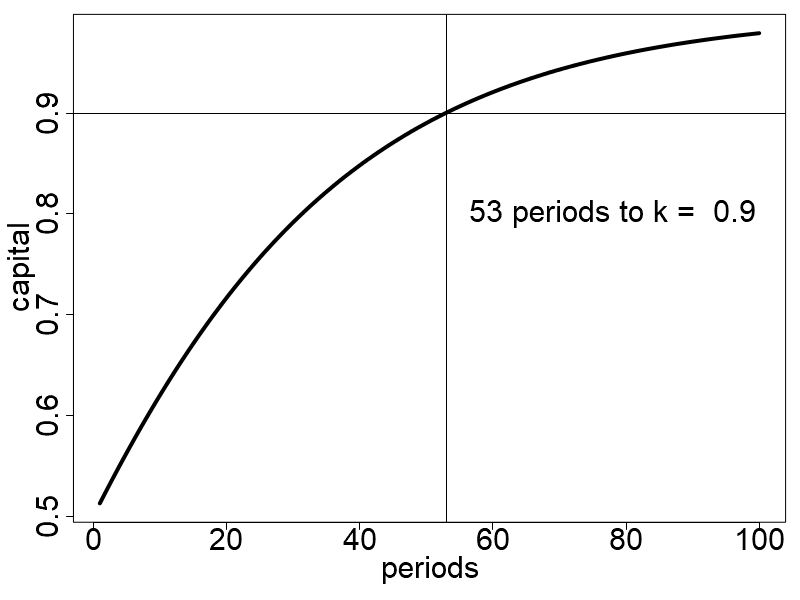
\includegraphics[width=0.5\linewidth]{solow_growth_alpha_high.png}
		\caption{Capital accumulation with $\alpha = 1/3$}
		\label{fig:cap_accumulation_alpha_high}
	\end{figure} 
	Notably, we see that it takes about twice as long for this economy to reach $k=0.9$ than the economy with $\alpha = 1/3$. Intuitively, this is because a higher level of $\alpha$ indicates that the production technology is more relatively more capital intensive, so it takes a longer amount of time to go from a low level of capital to $k=0.9$. 
\end{enumerate}




%\section*{Appendix - Matlab Code}
%\lstinputlisting{../Code/VFI_190313_1802.m}

\end{document}